\section{Two channels with response calibration}\label{sec:calibrated}
Calibration makes a source claim testable by limiting how much asymmetry the detectors can explain. A known test input bounds their relative phase, which then bounds their contribution to the observed asymmetry. Variance measures the size of fluctuations within one channel. For aligned recordings with variances $v_1,v_2$, consider
\begin{equation}
 \kappa=C_{12}(1)-C_{12}(-1).
 \label{eq:main-contrast}
\end{equation}
This contrast compares the covariance at one forward and one backward step. It is also the covariance between $Y_1(t)+Y_1(t+1)$ and $Y_2(t)-Y_2(t+1)$. Reversing the two observation times preserves the sum and changes the sign of the difference. Their covariance therefore gives a signed measure of the recorded time order. Other lags can remain asymmetric when this contrast is zero.

Suppose calibration supplies a bound on the relative response phase,
\begin{equation}
 r\ge\sup_\omega\left|\sin\omega\,
 \frac{\operatorname{Im}(H_1\overline H_2)}{|H_1H_2|}\right|.
 \label{eq:main-phase}
\end{equation}
The ratio is set to zero at a response zero. The supremum covers every allowed response and the source support. Under the reversible-source model,
\begin{equation}
 |\kappa|\le 2r\sqrt{v_1v_2}.\label{eq:main-tolerance}
\end{equation}
This is the maximum detector contribution allowed by the phase bound and the two variances. The factor $\sin\omega$ appears because the lag-one contrast weights the imaginary cross spectrum by that factor. The imaginary part records the component that changes sign when time order reverses. The factor gives greatest weight near $\omega=\pi/2$. For a reversible source, the cross-spectral measure $\mu_{12}$ is real, so
\begin{align*}
 |\kappa|&=2\left|\int\sin\omega\,\operatorname{Im}(H_1\overline H_2)\,d\mu_{12}\right|\\
 &\le2r\int |H_1H_2|\,|d\mu_{12}|\\
 &\le2r\sqrt{v_1v_2}.
\end{align*}
The last step uses positivity of the source spectral measure and Cauchy--Schwarz. Observation noise only increases the marginal variance scale. The factor two is sharp over the spectral-measure class, including line spectra (SM Sec.~S3.3). For the Brownian echo response, the exact-model value is $r\simeq0.0300$, giving a detector allowance near $0.0600\sqrt{v_1v_2}$. The implemented test uses an upper confidence bound from calibration, not this exact-response value.

\subsection{From a population tolerance to a finite-record test}
Equation~\eqref{eq:main-tolerance} limits the population contrast, the value defined by the underlying probability law rather than by one record. A finite estimate can exceed this value through sampling error, especially when successive observations are strongly dependent. We control that error through $\Gamma_N$, the covariance of the complete two-channel record, stacked by channel. We require
\begin{equation}
 \Gamma_N\preceq q\operatorname{diag}(v_1I_N,v_2I_N).
 \label{eq:main-envelope}
\end{equation}
The matrix inequality bounds the variance of every weighted sum of observations from either channel and any time in the record. We call this a covariance envelope. It prevents unaccounted dependence from making the uncertainty estimate too small. After each channel is divided by its standard deviation, $q$ bounds the largest eigenvalue of the complete record covariance. It therefore controls dependence between channels and across time throughout the record. Response calibration alone does not supply it.

One construction uses a source spectral floor and ceiling. If normalized source marginal densities obey $0<m_0\le g_i\le M_0$, define $\mathcal S=M_0/m_0$. If calibration bounds $\sup|H_i|^2/\|h_i\|_2^2$ by $\widehat C_i$, and the error spectra obey $f_{E,i}\le J_i\operatorname{Var}E_i$, then
\begin{equation}
 \widehat q=\max\{2\mathcal S\max_i\widehat C_i,\max_iJ_i\}
 \label{eq:main-q}
\end{equation}
is valid when the calibration confidence regions contain the true response coefficients. Here $h_i$ is the vector of response coefficients. The source ratio and the error bounds are supplied separately. Physical dynamics can also supply the full bound directly, as below.

The same covariance envelope must control estimation of both the contrast and its variance scale. For $N\ge3$, put $n=N-1$, $U_t=Y_1(t)+Y_1(t+1)$, and $W_t=Y_2(t)-Y_2(t+1)$. We estimate the contrast from their products. Unknown means require centering, so we subtract the sample means of $U_t$ and $W_t$ using the same $n$ starting times. For the scale, we turn each centered sample variance into an upper confidence bound. Such a bound is a procedure whose output covers the true variance with a stated probability over repeated recordings. Define
\begin{align}
 s_n&=n^{-1}\sum_{t=0}^{n-1}(U_t-\bar U)(W_t-\bar W),\label{eq:main-stat}\\
 V_i&=N^{-1}\sum_{t=0}^{N-1}(Y_i(t)-\bar Y_i)^2,\\
 c_N(q)&=1-q/N-2\sqrt{q\log(200)/N},\label{eq:main-c}\\
 D_i(q)&=V_i/c_N(q),\qquad D_{\rm g}(q)=\sqrt{D_1(q)D_2(q)}.
 \label{eq:main-d}
\end{align}
The denominator $c_N(q)$ accounts for how far a dependent sample variance can fall below the population variance. The resulting ceilings are used only when $c_N(q)>0$. On one event of probability at least $0.99$, both satisfy $D_i\ge v_i$. Their geometric mean therefore bounds $\sqrt{v_1v_2}$ and is no greater than the larger individual ceiling. A large but valid covariance envelope can make this denominator nonpositive and leave the test unavailable.

The threshold adds an allowance for detector-induced contrast to an allowance for sampling fluctuations. The variance ceilings set the scale of both terms. To bound the fluctuations, we write the centered contrast as a Gaussian quadratic form, a weighted sum of products of Gaussian observations. Its coefficient matrix has Frobenius norm $f_n$, given below. Two bounds on the covariance-weighted norm are available, so the radius uses their smaller value:
\begin{align}
 f_n^2&=\frac{2n+2-4/n-4/n^2}{2n^2},\\
 R(q,D,N,t)&=2D\min\{qf_n,\sqrt{2qN}/n\}\sqrt t
                  +2qDt/n.\label{eq:main-radius}
\end{align}
\begin{theorem}[Calibrated test]\label{thm:main-complete}
Assume the stationary Gaussian observation model and a simultaneous calibration event of probability at least $0.99$ on which $\widehat r\ge r$ and $\widehat q\ge q$. The rule rejects when $c_N(\widehat q)>0$ and
\begin{equation}
 |s_n|>D_{\rm g}(\widehat q)\,2\widehat r+
 R(\widehat q,D_{\rm g}(\widehat q),N,\log(2/0.03)).
 \label{eq:main-test}
\end{equation}
Its rejection probability under the stated reversible-source model is at most $0.05$. The error allocations are $0.01$ for calibration, $0.01$ for variance coverage, and $0.03$ for the statistic.
\end{theorem}

In words, reject only when the observed lag contrast exceeds the calibrated detector allowance plus a sampling margin. Under any allowed reversible-source model, this rule falsely rejects in at most five percent of repeated experiments. This is an error guarantee for the procedure, not a probability that the source is reversible after a particular result. The threshold has the form \emph{variance scale $\times$ (detector allowance + sampling allowance)}. More samples can reduce sampling error, but cannot remove the allowed detector contribution. Common centering preserves the detector tolerance because it multiplies the spectral integrand by an even nonnegative factor. Gaussian quadratic-form bounds then give the radius. The fitted threshold is at least a fixed valid threshold on the calibration and variance-coverage events, so fitting requires no additional independence assumption. SM Sec.~S4.5, Theorem~S7 and Lemmas~S2--S3 prove the result.

\begin{table}[t]
\caption{Error allocations explain the logarithms in the thresholds. Each column totals $0.05$. The fitted-source bank has $M$ fixed filters.}\label{tab:budget}
\begin{ruledtabular}\begin{tabular}{lcc}
Component & Calibrated pair & Fitted-source bank\\
Source confidence & --- & $0.005$\\
Calibration & $0.01$ & $0.01$\\
Both variance ceilings & $0.01$ & $0.01$\\
Contrast & $0.03$ & $0.025$\\\hline
Variance logarithm & $\log(200)$ & $\log(200M)$\\
Contrast logarithm & $\log(2/0.03)$ & $\log(80M)$\\
\end{tabular}\end{ruledtabular}
\end{table}

Calibration uses known deterministic inputs and a full-rank response design at fixed integer coefficient positions. Errors are independent Gaussian values with a common positive variance within each channel, and residual degrees of freedom are positive. Responses must stay unchanged between calibration and testing. Coefficient confidence regions and derivative bounds between grid points give an all-frequency phase allowance (SM Secs.~S3.4--S3.5). Table~\ref{tab:budget} gives the total false-rejection budget. Bounded rounding is covered by enlarging the variance ceilings and adding a deterministic contrast error (SM Sec.~S4.5, Proposition~S7).

\subsection{Calibrated inference for the Brownian gyrator}\label{sec:physical}
The Brownian model tests both requirements of source inference: allowing an equilibrium detector effect and detecting a driven source. For the family $1\le T_i\le4$, the drift in Eq.~\eqref{eq:ou-model} has smallest eigenvalue $1/2$. Its covariance obeys $(2/3)I\preceq\Sigma\preceq8I$, and $\|e^{-Ak}\|\le e^{-k/2}$. Together with the response filters, these family bounds give $q=56$ for every tested temperature (SM Sec.~S7.2). This envelope is deliberately common to equilibrium and driven records.

Figure~\ref{fig:study-brownian} places the different targets side by side. The calibrated test gives no equilibrium rejection at any length. Raw block-bootstrap detections instead rise from $87/400$ through $271/400$ to $397/400$. They detect the recorded asymmetry permitted by the equilibrium source and its unequal sensors. Interpreting these raw detections as source irreversibility would therefore become increasingly misleading as data accumulate.

The same valid envelope has a substantial sensitivity cost. The calibrated test detects all $200$ fourfold-temperature records only at $N=524289$, and detects none at temperature ratio two throughout the tested range. The generating entropy-production rates are $9/32$ and $1/16$, respectively, in units of $k_B$ per unit time. Here $k_B$ is Boltzmann's constant. These rates describe the simulated source; the test does not estimate them. A relaxation time measures how long a fluctuation takes to decay by a factor of $e$. The slowest relaxation time is only two sampling intervals, so the longest record exceeds $260000$ relaxation times. Thus this example is limited by a conservative family envelope as well as by correlation.

An exact-response population calculation explains the scale of this cost without changing any study decision. At $N=524289$ and $q=56$, the normalized detector and sampling allowances are approximately $0.0600$ and $0.0608$. Correcting the variance scale gives a threshold near $0.1268$. The recorded normalized contrasts at temperature ratios two and four are approximately $0.0915$ and $0.1849$. These analytic reference values omit calibration and recording increments; they explain why a valid family bound can obscure the weaker alternative. The saved study retains $q=56$ throughout.

\begin{figure*}[t]\centering
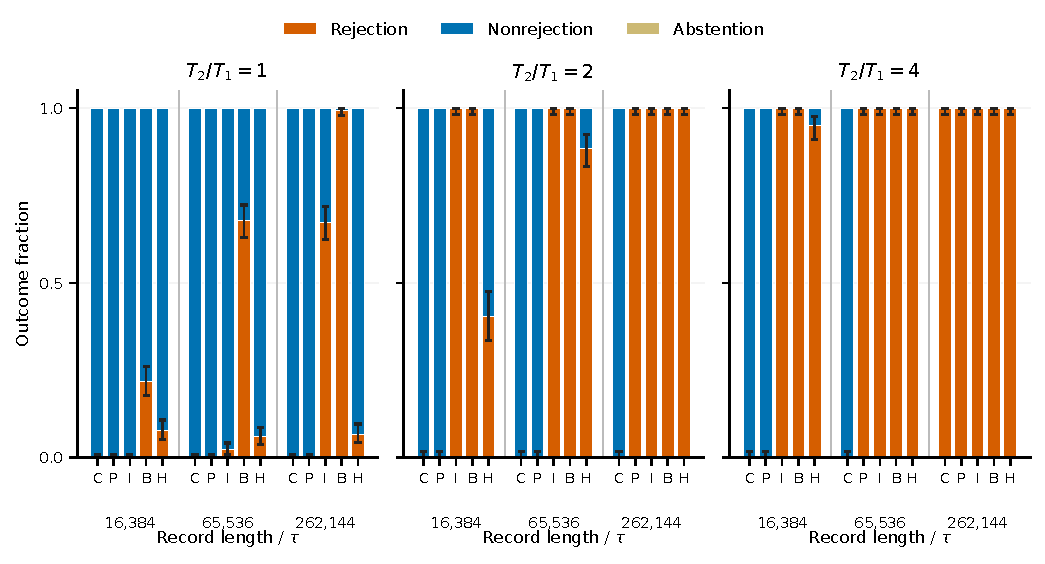
\includegraphics[width=\textwidth]{figures/brownian_operating_compact.pdf}
\caption{Raw bootstrap detections reach $397/400$ at equilibrium, while the calibrated source test rejects $0/400$. Temperature ratios are 1, 2, and 4; lengths are $N/2$ relaxation times. Methods: C, calibrated; P, phase ignored; I, independent windows; B, moving-block bootstrap; H, imaginary coherency. Equilibrium cells have 400 records; alternatives have 200. Bars give pointwise 95\% binomial intervals. Raw methods test recorded asymmetry; C tests source reversibility under response information. No method abstains. Values are saved study results.}\label{fig:study-brownian}
\end{figure*}

\begin{table*}[t]
\caption{Comparison targets. An approximate test for recorded asymmetry is not a finite-sample test for source reversibility under unequal sensors.}\label{tab:comparators}
\begin{ruledtabular}\begin{tabular}{>{\raggedright\arraybackslash}p{.20\textwidth}>{\raggedright\arraybackslash}p{.32\textwidth}>{\raggedright\arraybackslash}p{.19\textwidth}>{\raggedright\arraybackslash}p{.20\textwidth}}
Procedure & Null restriction & Detector information & Guarantee here\\
Calibrated contrast & Reversible source within the allowed response model & Relative phase and full covariance bound & Finite false-rejection bound\\
Spectral cycle & Real source cross spectra under sampled diagonal responses & Factorization; covariance and tail bounds & Finite false-rejection bound\\
Independent-window lag rule & Zero recorded lag contrast & None & Ignores overlapping-window dependence\\
Moving-block bootstrap & Zero recorded lag contrast & None in raw form & Approximate bootstrap\\
Imaginary coherency & Zero imaginary normalized cross spectrum & None & Approximate segment bootstrap\\
Phase-adjusted comparators & Recorded contrast within a detector allowance & Same phase bound as calibrated rule & No finite source-null guarantee here\\
\end{tabular}\end{ruledtabular}
\end{table*}
Table~\ref{tab:comparators} states the comparison targets before interpreting their rejection fractions. SM Secs.~S8.5 and S9.4 give their definitions and the phase-boundary controls.
